\chapter{2D case}

\section{Problem}
In this part, we will focus on a 2D point cloud and we will use for the energy
the area of the $ r $-offset of a point cloud $ X $: the Minkowski sum with an euclidean
ball $ B(0, r) $. This offset will be denoted by $ X^{\oplus r} $.

\section{Area of a union of balls}
In order to compute this energy, we need to know how to estimate the area of the
intersection of a ball and a Voronoi cell. Indeed, the area of the union of
balls is the same as the sum of the areas of the restrictions of the balls to
their Voronoi cell (because essentially the Voronoi cells partition the plane).

This is the same work as the one done in \cite{cazals2011computing} except that
we restrict ourselves to 2D which is simpler than in 3D.

For doing that, we need to decompose the intersection into triangles and
spherical caps.

The following figure illustrates the different cases for the intersection of a
Voronoi cell and a ball in 2D:
\begin{figure}[H]
    \centering
    \begin{minipage}{0.32\linewidth}
        \centering
        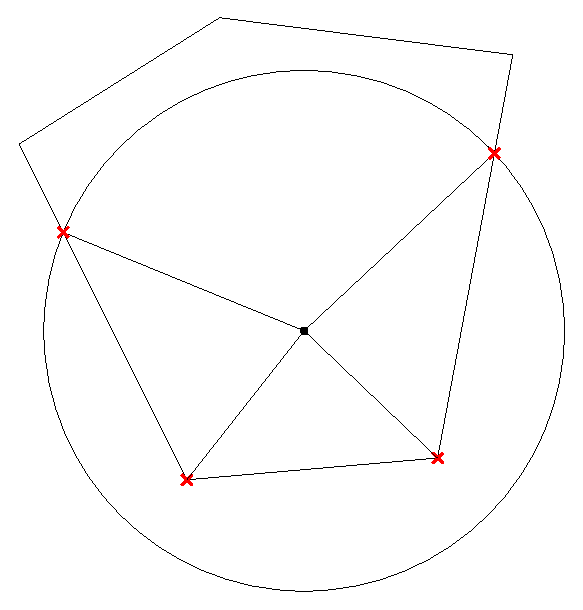
\includegraphics[scale=0.4]{inter_voronoi_ball_2d}
        \subcaption{General case}
        \label{fig:inter_voronoi_ball_2d:a}
    \end{minipage}
    \begin{minipage}{0.32\linewidth}
        \centering
        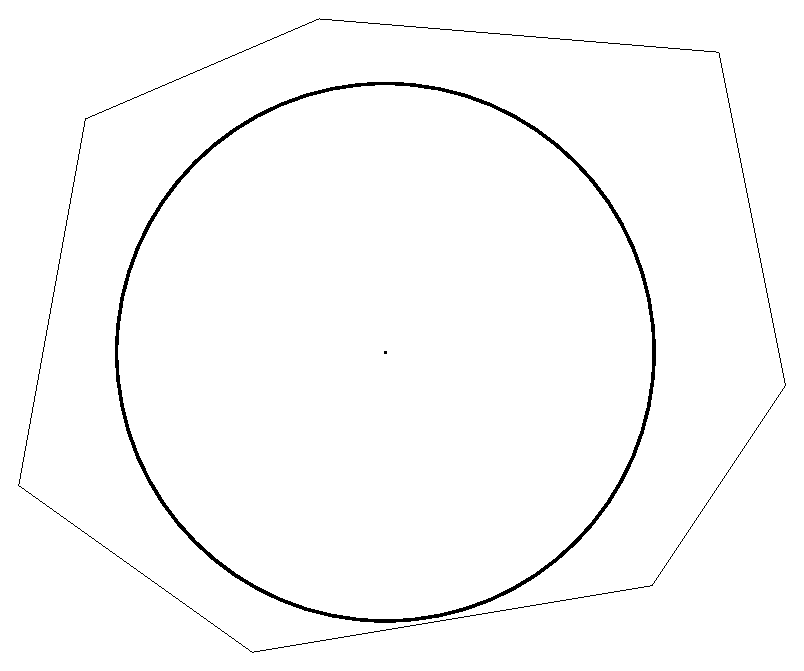
\includegraphics[scale=0.4]{inter_voronoi_ball_2d_no_inter}
        \subcaption{No intersections}
        \label{fig:inter_voronoi_ball_2d:b}
    \end{minipage}
    \begin{minipage}{0.32\linewidth}
        \centering
        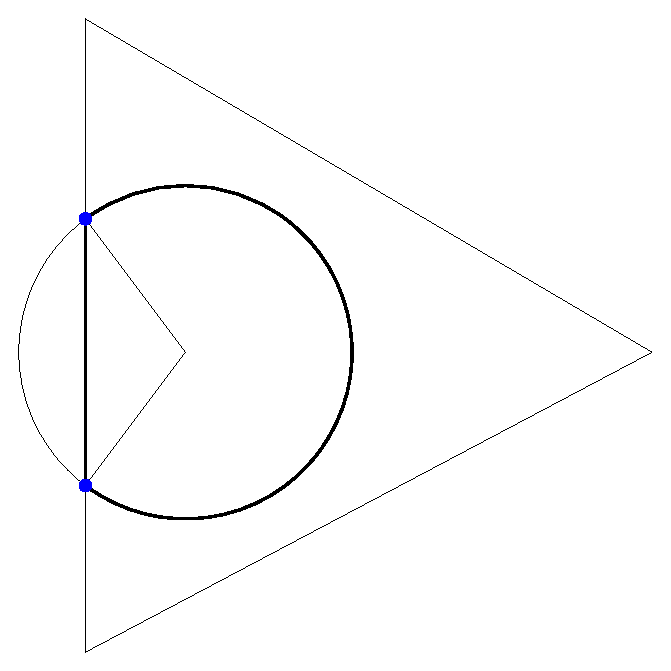
\includegraphics[scale=0.4]{inter_voronoi_ball_2d_2_inter}
        \subcaption{2 intersections}
        \label{fig:inter_voronoi_ball_2d:c}
    \end{minipage}

   \caption{Different cases for the intersection between a Voronoi cell and a sphere}
   \label{fig:inter_voronoi_ball_2d}
\end{figure}

We used \texttt{CGAL} to compute the Delaunay triangulation of our point set.
Given this triangulation, we can compute the Voronoi cell of a point by doing
the following:
\begin{enumerate}
    \item Access the neighbouring faces of a vertex using the
        \texttt{incident\_faces} method.
    \item Compute the Voronoi vertices of these faces using the \texttt{dual}
        method.
\end{enumerate}

Then, we will need to know the vertices of the boundary of the intersection (the
points forming the bold boundary in \ref{fig:inter_voronoi_ball_2d}). There are
two types of those points: some are Voronoi vertices and some are intersections
of Voronoi edges and circles. To each of these points, we attach a boolean
saying whether the point is an interior point or an intersection one. We also
attach the corresponding Voronoi edge.

Then, we loop over the Voronoi edges $ e = pq $ of a vertex $ v $:
\begin{itemize}
    \item if $ p $ and $ q $ are interior points, we add the triangle $ pvq $.
    \item if $ p $ or $ q $ is interior point, we add the triangle $ pvq $.
    \item if $ p $ and $ q $ are intersection points, then if they belong to the
        same Voronoi edge, we add the triangle $ pvq $. If not, we add the
        angular sector $ \vec{vp}, \vec{vq} $.
\end{itemize}

Some special cases need to be handled:
\begin{itemize}
    \item the boundary of the Voronoi cell is entirely outside the ball, then we
        add $ \pi r^2 $ to the area of the union (see
        \ref{fig:inter_voronoi_ball_2d:b}).
    \item the boundary consists of two intersection points $ p $ and $ q $, then
        we add the triangle $ pvq $ and the angular sector $ \vec{vp}, \vec{vq}
        $ (see \ref{fig:inter_voronoi_ball_2d:c}).
    \item there is only one point on the boundary (can happen if adjacent balls
        are tangential), then we add $ \pi r^2 $.
\end{itemize}

We used the same techniques for computing the perimeter of the boundary of the
intersection except that if there are no intersection then the perimeter is null
and instead of adding triangles areas or angular sectors, we add lengths of
circular arcs.

% TODO

\section{Gradient}

Then, we used the automatic differentiation to compute the gradient of the
previously computed area.

Here are a few examples of such gradients for different input point sets:

\begin{figure}[H]
    \centering

    \begin{minipage}{0.8\linewidth}
        \centering
        \includegraphics[scale=0.32]{ellipse-200-001-100}
        \includegraphics[scale=0.32]{ellipse-200-001-100-gradients}
        \subcaption{200 samples on an ellipse with $ r = 100 $}
        \label{fig:gradients_2d_ellipse}
    \end{minipage}

    \begin{minipage}{0.8\linewidth}
        \centering
        \includegraphics[scale=0.32]{circle-120-001-100}
        \includegraphics[scale=0.32]{circle-120-001-100-gradients}
        \subcaption{120 samples on a circle with $ r = 100 $}
        \label{fig:gradients_2d_ellipse}
    \end{minipage}

    \begin{minipage}{0.8\linewidth}
        \centering
        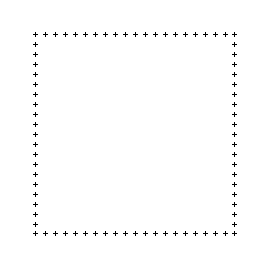
\includegraphics[scale=0.32]{square-76-001-100}
        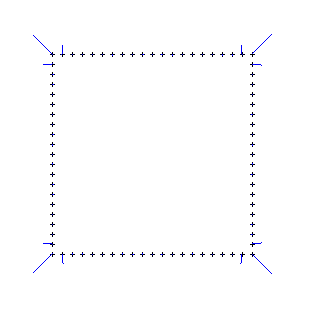
\includegraphics[scale=0.32]{square-76-001-100-gradients}
        \subcaption{76 samples on a square with $ r = 100 $}
        \label{fig:gradients_2d_ellipse}
    \end{minipage}

    \caption{Input point set / Normalized computed gradients}
    \label{fig:gradients_2d}
\end{figure}

In the previous screenshots, we can see that the gradients are (if the radius of
the balls are big enough and if the sampling is uniform) in the same direction
that the normals to the underlying surface.

% TODO

\section{Gradient descent}

Then, as said in the introduction, we will approximate the mean curvature flow
by applying a gradient descent algorithm where the considered energy is the area
(or the perimeter of the boundary) of the union of balls.

This gradient descent will be done using a constant timestep (Euler explicit
scheme).

We needed to choose "good" weights for the gradient descent. Indeed, in a normal
mean curvature flow, all the points move with the same distance related to the
curvature. But here, this may not be the case since the energy depends on the
curvature of our restricted region.

One way to avoid this problem is to weight the gradient by the perimeter of the
visible part of the restricted region. But by doing that, we can divide by $ 0 $
so we need to choose the time step according to these weights in order to avoid
the case where a point does not see anything.

% TODO

\section{Experiments}

We did some experiments to validate our results. The fist thing we did was to
apply our flow to a set of points randomly and/or uniformly sampled on an ellipse.

Then, we added some noise on these points to test the robustness of our
algorithm.

% TODO: figures

We also compare the two gradient flows: using the area or the perimeter of the
boundary.

We notice that the gradient flow of the area may create holes in the point set
which is not the case for the gradient flow of the perimeter.

% TODO: explain why

We remark that if the time step is too large then the algorithm does not
converge ($ 0.1 $ for example).

% Union of balls
% Intersection with Voronoi cells
% Volume
% Gradient descent: weights
% Experiments

% vim: set spelllang=en :
